% Created by tikzDevice version 0.6.2-92-0ad2792 on 2012-09-16 00:28:59
% !TEX encoding = UTF-8 Unicode
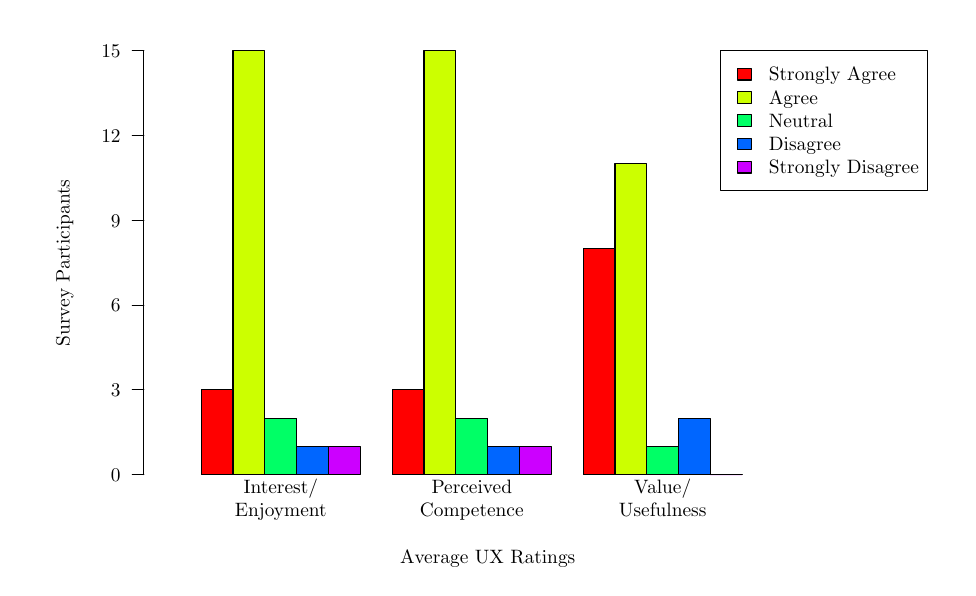
\begin{tikzpicture}[x=1pt,y=1pt]
\definecolor[named]{fillColor}{rgb}{1.00,1.00,1.00}
\path[use as bounding box,fill=fillColor,fill opacity=0.00] (0,0) rectangle (332.44,195.13);
\begin{scope}
\path[clip] (  0.00,  0.00) rectangle (332.44,195.13);
\definecolor[named]{drawColor}{rgb}{0.00,0.00,0.00}
\definecolor[named]{fillColor}{rgb}{1.00,0.00,0.00}

\path[draw=drawColor,line width= 0.4pt,line join=round,line cap=round,fill=fillColor] ( 62.70, 33.60) rectangle ( 74.21, 64.23);
\definecolor[named]{fillColor}{rgb}{0.80,1.00,0.00}

\path[draw=drawColor,line width= 0.4pt,line join=round,line cap=round,fill=fillColor] ( 74.21, 33.60) rectangle ( 85.71,186.73);
\definecolor[named]{fillColor}{rgb}{0.00,1.00,0.40}

\path[draw=drawColor,line width= 0.4pt,line join=round,line cap=round,fill=fillColor] ( 85.71, 33.60) rectangle ( 97.21, 54.02);
\definecolor[named]{fillColor}{rgb}{0.00,0.40,1.00}

\path[draw=drawColor,line width= 0.4pt,line join=round,line cap=round,fill=fillColor] ( 97.21, 33.60) rectangle (108.71, 43.81);
\definecolor[named]{fillColor}{rgb}{0.80,0.00,1.00}

\path[draw=drawColor,line width= 0.4pt,line join=round,line cap=round,fill=fillColor] (108.71, 33.60) rectangle (120.21, 43.81);
\definecolor[named]{fillColor}{rgb}{1.00,0.00,0.00}

\path[draw=drawColor,line width= 0.4pt,line join=round,line cap=round,fill=fillColor] (131.72, 33.60) rectangle (143.22, 64.23);
\definecolor[named]{fillColor}{rgb}{0.80,1.00,0.00}

\path[draw=drawColor,line width= 0.4pt,line join=round,line cap=round,fill=fillColor] (143.22, 33.60) rectangle (154.72,186.73);
\definecolor[named]{fillColor}{rgb}{0.00,1.00,0.40}

\path[draw=drawColor,line width= 0.4pt,line join=round,line cap=round,fill=fillColor] (154.72, 33.60) rectangle (166.22, 54.02);
\definecolor[named]{fillColor}{rgb}{0.00,0.40,1.00}

\path[draw=drawColor,line width= 0.4pt,line join=round,line cap=round,fill=fillColor] (166.22, 33.60) rectangle (177.72, 43.81);
\definecolor[named]{fillColor}{rgb}{0.80,0.00,1.00}

\path[draw=drawColor,line width= 0.4pt,line join=round,line cap=round,fill=fillColor] (177.72, 33.60) rectangle (189.22, 43.81);
\definecolor[named]{fillColor}{rgb}{1.00,0.00,0.00}

\path[draw=drawColor,line width= 0.4pt,line join=round,line cap=round,fill=fillColor] (200.73, 33.60) rectangle (212.23,115.27);
\definecolor[named]{fillColor}{rgb}{0.80,1.00,0.00}

\path[draw=drawColor,line width= 0.4pt,line join=round,line cap=round,fill=fillColor] (212.23, 33.60) rectangle (223.73,145.89);
\definecolor[named]{fillColor}{rgb}{0.00,1.00,0.40}

\path[draw=drawColor,line width= 0.4pt,line join=round,line cap=round,fill=fillColor] (223.73, 33.60) rectangle (235.23, 43.81);
\definecolor[named]{fillColor}{rgb}{0.00,0.40,1.00}

\path[draw=drawColor,line width= 0.4pt,line join=round,line cap=round,fill=fillColor] (235.23, 33.60) rectangle (246.73, 54.02);
\definecolor[named]{fillColor}{rgb}{0.80,0.00,1.00}

\path[draw=drawColor,line width= 0.4pt,line join=round,line cap=round,fill=fillColor] (246.73, 33.60) rectangle (258.24, 33.60);
\end{scope}
\begin{scope}
\path[clip] (  0.00,  0.00) rectangle (332.44,195.13);
\definecolor[named]{drawColor}{rgb}{0.00,0.00,0.00}

\node[text=drawColor,anchor=base,inner sep=0pt, outer sep=0pt, scale=  0.70] at ( 91.46, 26.88) {Interest/};

\node[text=drawColor,anchor=base,inner sep=0pt, outer sep=0pt, scale=  0.70] at ( 91.46, 18.48) {Enjoyment};

\node[text=drawColor,anchor=base,inner sep=0pt, outer sep=0pt, scale=  0.70] at (160.47, 26.88) {Perceived};

\node[text=drawColor,anchor=base,inner sep=0pt, outer sep=0pt, scale=  0.70] at (160.47, 18.48) {Competence};

\node[text=drawColor,anchor=base,inner sep=0pt, outer sep=0pt, scale=  0.70] at (229.48, 26.88) {Value/};

\node[text=drawColor,anchor=base,inner sep=0pt, outer sep=0pt, scale=  0.70] at (229.48, 18.48) {Usefulness};
\end{scope}
\begin{scope}
\path[clip] (  0.00,  0.00) rectangle (332.44,195.13);
\definecolor[named]{drawColor}{rgb}{0.00,0.00,0.00}

\node[text=drawColor,anchor=base,inner sep=0pt, outer sep=0pt, scale=  0.70] at (166.22,  1.68) {Average UX Ratings};

\node[text=drawColor,rotate= 90.00,anchor=base,inner sep=0pt, outer sep=0pt, scale=  0.70] at ( 15.12,110.16) {Survey Participants};
\end{scope}
\begin{scope}
\path[clip] (  0.00,  0.00) rectangle (332.44,195.13);
\definecolor[named]{drawColor}{rgb}{0.00,0.00,0.00}

\path[draw=drawColor,line width= 0.4pt,line join=round,line cap=round] ( 42.00, 33.60) -- ( 42.00,186.73);

\path[draw=drawColor,line width= 0.4pt,line join=round,line cap=round] ( 42.00, 33.60) -- ( 37.80, 33.60);

\path[draw=drawColor,line width= 0.4pt,line join=round,line cap=round] ( 42.00, 64.23) -- ( 37.80, 64.23);

\path[draw=drawColor,line width= 0.4pt,line join=round,line cap=round] ( 42.00, 94.85) -- ( 37.80, 94.85);

\path[draw=drawColor,line width= 0.4pt,line join=round,line cap=round] ( 42.00,125.48) -- ( 37.80,125.48);

\path[draw=drawColor,line width= 0.4pt,line join=round,line cap=round] ( 42.00,156.10) -- ( 37.80,156.10);

\path[draw=drawColor,line width= 0.4pt,line join=round,line cap=round] ( 42.00,186.73) -- ( 37.80,186.73);

\node[text=drawColor,anchor=base east,inner sep=0pt, outer sep=0pt, scale=  0.70] at ( 33.60, 31.19) {0};

\node[text=drawColor,anchor=base east,inner sep=0pt, outer sep=0pt, scale=  0.70] at ( 33.60, 61.82) {3};

\node[text=drawColor,anchor=base east,inner sep=0pt, outer sep=0pt, scale=  0.70] at ( 33.60, 92.44) {6};

\node[text=drawColor,anchor=base east,inner sep=0pt, outer sep=0pt, scale=  0.70] at ( 33.60,123.07) {9};

\node[text=drawColor,anchor=base east,inner sep=0pt, outer sep=0pt, scale=  0.70] at ( 33.60,153.69) {12};

\node[text=drawColor,anchor=base east,inner sep=0pt, outer sep=0pt, scale=  0.70] at ( 33.60,184.32) {15};
\end{scope}
\begin{scope}
\path[clip] (  0.00,  0.00) rectangle (332.44,195.13);
\definecolor[named]{drawColor}{rgb}{0.00,0.00,0.00}

\path[draw=drawColor,line width= 0.4pt,line join=round,line cap=round] (250.19,186.73) rectangle (325.19,136.33);
\definecolor[named]{fillColor}{rgb}{1.00,0.00,0.00}

\path[draw=drawColor,line width= 0.4pt,line join=round,line cap=round,fill=fillColor] (256.49,180.43) rectangle (261.53,176.23);
\definecolor[named]{fillColor}{rgb}{0.80,1.00,0.00}

\path[draw=drawColor,line width= 0.4pt,line join=round,line cap=round,fill=fillColor] (256.49,172.03) rectangle (261.53,167.83);
\definecolor[named]{fillColor}{rgb}{0.00,1.00,0.40}

\path[draw=drawColor,line width= 0.4pt,line join=round,line cap=round,fill=fillColor] (256.49,163.63) rectangle (261.53,159.43);
\definecolor[named]{fillColor}{rgb}{0.00,0.40,1.00}

\path[draw=drawColor,line width= 0.4pt,line join=round,line cap=round,fill=fillColor] (256.49,155.23) rectangle (261.53,151.03);
\definecolor[named]{fillColor}{rgb}{0.80,0.00,1.00}

\path[draw=drawColor,line width= 0.4pt,line join=round,line cap=round,fill=fillColor] (256.49,146.83) rectangle (261.53,142.63);

\node[text=drawColor,anchor=base west,inner sep=0pt, outer sep=0pt, scale=  0.70] at (267.83,175.92) {Strongly Agree};

\node[text=drawColor,anchor=base west,inner sep=0pt, outer sep=0pt, scale=  0.70] at (267.83,167.52) {Agree};

\node[text=drawColor,anchor=base west,inner sep=0pt, outer sep=0pt, scale=  0.70] at (267.83,159.12) {Neutral};

\node[text=drawColor,anchor=base west,inner sep=0pt, outer sep=0pt, scale=  0.70] at (267.83,150.72) {Disagree};

\node[text=drawColor,anchor=base west,inner sep=0pt, outer sep=0pt, scale=  0.70] at (267.83,142.32) {Strongly Disagree};
\end{scope}
\end{tikzpicture}
